\documentclass[12pt,a4paper,fleqn]{article}

\usepackage{ucs}
\usepackage[utf8x]{inputenc}
\usepackage[T2A]{fontenc}
\usepackage[english,russian]{babel}

\usepackage{textcomp}
\usepackage{indentfirst}
\usepackage{verbatim}
\usepackage{amsthm}
\usepackage{amssymb}
\usepackage{amsmath}
\usepackage{graphicx}

\usepackage[left=20mm,right=20mm,top=20mm,bottom=20mm]{geometry}

\usepackage{listings}
% Значения по умолчанию для listings
\lstset{
  basicstyle=\footnotesize,
  frame=none,
  breakatwhitespace=true,% разрыв строк только на whitespacce
  breaklines=true,       % переносить длинные строки
  captionpos=b,          % подписи снизу
  numbers=none,          % без нумерации
  showspaces=false,      % показывать пробелы подчеркиваниями -- идиотизм 70-х годов
  showstringspaces=false,
  showtabs=false,        % и табы тоже
  stepnumber=1,
  tabsize=4              % кому нужны табы по 8 символов?..
}

\sloppy
\hyphenpenalty=9000

\makeatletter
\renewcommand\@biblabel[1]{\hfill#1.}
\makeatother

\pagestyle{empty}

\begin{document}

\begin{center}
\huge Параллельная проверка утверждений для моделей конечных детерменированных систем
\end{center}

\vspace{5mm}

\begin{center}
И.А.~Коротков, В.А.~Крищенко\\
\it Московский государственный технический университет им.~Н.~Э.~Баумана\\\
\rm
Россия, 105005, Москва, 2-ая Бауманская, 5\\
E-mail: kva@bmstu.ru

\hspace{1.25cm}

\vspace{8mm}

\begin{minipage}{12.16cm}\noindent

\footnotesize{\bf Ключевые слова:} формальная верификация, проверка моделей, генерация состояний, параллельные
вычисления, Promela

\noindent{\bf Key words:} model checking, state generation, parallel statespace, parallelism, Promela

\vspace{6mm}

\noindent Основной проблемой верификации конечных моделей является комбинаторный <<взрыв>> числа состояний, которые с
ростом размера модели становится затруднительно хранить в ОЗУ одной машины. Рассматривается подход к верификации
конечных моделей на основе параллельной генерации состояний и их распределенного хранения. Предлагается схема
распределенного хранения состояний, позволяющая уменьшить число удаленных вызовов между узлами в процессе
генерации. Приводятся результаты экспериментов, полученные при помощи разработанного программного средства.

\vspace{4mm}

\noindent {\bf Parallel statespace generation during model-checking for systems with distributed memory} /
I.\,A.\,Korotkov (Moscow State Technical Univercity, 5 Baumanskay 2-aya ul., Moscow 105005, Russia,
e-mail:~korotkov2@mail.ru).

Major limitation of model checking is statespace combinatorial explosion, which makes even medium-sized model
inappropriate for that kind of verification. In this paper, parallel statespace generation with distributed state
storage is proposed as a possible solution. State partitioning scheme that allows to reduce number of remote calls
during generation process is developed.  Experimental results, produced by developed verification tool, are given and
prove that proposed partitioning scheme is better than random uniform distribution.
\end{minipage}

\end{center}

\section{Введение}
\label{sec:intro}

При разработке сложных параллельных систем (систем, состоящих из нескольких асинхронно работающих компонент) с высокой
степенью надежности традиционных подходов к тестированию зачастую бывает недостаточно, поскольку они позволяет выявить
лишь легко воспроизводимые ошибки. В некоторых случаях, например, в программном обеспечении для бортовых систем,
определенные классы ошибок требуется полностью исключить.

Для таких случаев применяется проверка модели (model checking)~--- автоматический формальный подход, при котором на основе
дискретной детерминированной модели программы или комплекса программ строится полное пространство состояний и на нем
проверяется набор интересующих нас утверждений~--- спецификация~\cite{Clarke}. Проверку моделей можно использовать для
поиска взаимоблокировок в параллельных алгоритмах и ошибок в спецификациях сетевых протоколов. В качестве примера можно
привести протокол маршрутизации RIP: проверка модели сети из четырех маршрутизаторов, соединенных четыремя сетевыми
интерфейсами, на предмет возникновения циклов в маршрутных таблицах позволяет убедиться, что существуют сценарии, при
которых такие циклы возникают, и необходимо использование специальных мер (расщепленный горизонт) для их
избежания~\cite{RipOnSpin}.

\section{Формальное описание проверки конечных моделей}
\label{sec:modelchecking}

Пространство состояний моделируемой программы или программного комплекса можно формализовать, как модель Крипке
(структуру Крипке, Kripke structure)~\cite{Clarke}. Моделью Крипке $M$ над множеством атомарных высказываний $AP$
называют четверку $(S, S_0, R, L)$, где:

\begin{itemize}
\item $S$~--- конечное множество состояний;
\item $S_0 \in S$~--- множество начальных состояний;
\item $R \in S \times S$~--- отношение переходов, которые обязано быть тотальным, т.е. для каждого состояния $s \in S$
  должно существовать такое состояние $s' \in S$, что имеет место $R(s, s')$;
\item $L\colon S \rightarrow 2^{AP}$~--- функция, которая помечает каждое состояние множеством  атомарных высказываний, истинных в этом состоянии.
\end{itemize}

Путь в модели $M$ из состояния $s$~--- это бесконечная последовательность состояний $\pi = s_0 s_1 \ldots$, такая, что
$s_o = s$ и для всех $i \geq 0$ выполняется $R(s_i, s_{i+1})$.

Моделируемый программный комплекс в каждом своем состоянии описываются набором значений переменных $V = \{v_0, v_1,
\ldots\}$, принимающих значения на конечном множестве $D$ (домене интерпретации) и описывающих отдельные компоненты и
взаимодействие между ними. Множество $AP$ состоит из утверждений вида $v_i = d_i$, где $d_i \in D$. Таким образом,
каждое состояние $s$ в $M$ представляет собой отображение $V \rightarrow D$.

Отношение $R$ определяется следующим образом. Пусть имеются два состояния, $s_1$ и $s_2$. Если в $s_1$ имеется
компонент, который может выполнить атомарный переход (изменение значений своих переменных), в результате выполнения
которого система будет находиться в состоянии $s_2$, тогда состояния $s_1$ и $s_2$ связаны отношением перехода: $(s_1,
s_2) \in R$. В случае, если нет такого состояния $s_2$, для которого бы выполнялось $R(s_1, s_2)$, полагается $R(s_1,
s_1)$, т.е. <<тупиковое>> состояние связано отношение перехода само с собой.

Для формализации проверяемых на модели $M$ утверждений обычно используются временные логики~--- LTL (linear time logic,
логика линейного времени), CTL (computation tree logic, логика ветвящегося времени), CTL* (объединение LTL и
CTL)~\cite{Clarke, Velder}. Формулы в CTL* составляются из атомарных утверждений относительно значений переменных $v_i$
и кванторов: $\mathbf{A}$ (all)~--- <<для всех путей, выходящих из данного состояния>>, $\mathbf{E}$ (exists)~---
<<существует такой путь, выходящий из данного состояния>>, $\mathbf{F}$ (finally)~--- <<рано или поздно в пути
встретится состояние, в котором выполняется ...>>, $\mathbf{G}$ (globally)~--- <<во всех состояниях пути выполняется
...>>, $\mathbf{X}$ (next)~--- <<в следующем состояния на данном пути выполняется ...>>, $\mathbf{U}$ (until)~--- <<пока
в пути не появится состояние, в котором выполняется $y$, во всех состояниях должно выполняться $x$>>.

Например, формула $\mathbf{AFG}~x$ означает <<во всех путях, идущих из начального состояния, с некоторого состояния на протяжении всего
пути выполняется $x$>>, а формула $\mathbf{AGEF}~x$ означает <<во всех путях, идущих из начального состояния, из каждого состояния есть хотя бы
один путь, в котором рано или поздно встретится состояние, в котором выполняется $x$>>.

\section{Средство проверки конечных модели SPIN}
\label{sec:spin}

Наиболее распространенным средством проверки конечных моделей является ПО SPIN, использующее для описания исходной
модели язык \emph{Promela} (PROtocol Meta Language)~\cite{SpinRoot}.

Модель на языке Promela~ описывается в виде набора процессов, состоящих из последовательности команд. Каждый процесс
имеет свой набор локальных переменных (в том числе счетчик команд). Для взаимодействия между процессами могут
использоваться глобальные переменные и каналы (очереди сообщений). Каждая команда имеет свое условие выполнимости, и
процесс считается заблокированным, если условие выполнимости его текущей команды не выполнено.

Пример описания модели семафора Дейкстры~\cite{SPIN} и трех захватывающих его процессов в нотации Promela привен ниже:

\begin{lstlisting}[language=Promela]
mtype { p, v };
chan sema = [0] of { mtype };
active proctype Dijkstra()
{      byte count = 1;
       do
       :: (count == 1) ->
               sema!p; count--
       :: (count == 0) ->
               sema?v; count++
       od
}
active [3] proctype user()
{       do
        :: enter: sema?p;  /* enter critical section */
            crit: skip;    /* critical section */
                  sema!v;  /* leave critical section */
        od
}
\end{lstlisting}

В ходе верификации SPIN выполняет исчерпывающий поиск в глубину по графу состояний (модели Крипке) и, при обнаружении
пути, на котором нарушается проверяемое утверждение, сохраняет его в качестве контрпримера~\cite{Clarke}. Если
контрпример обнаружить не удается, верификация успешна. Функциональная схема процесса проверки модели изображена на
рис.~\ref{fig:modelchk-idef0-a0}.

\begin{figure}[ht]
  \centering
  \includegraphics[width=\textwidth]{../graphics/modelchk-idef0-a0}
  \caption{Функциональная схема проверки модели}
  \label{fig:modelchk-idef0-a0}
\end{figure}

\section{Параллельная генерация состояний}
\label{sec:pargen}

При росте числа и сложности компонент моделируемого программного комплекса наблюдается комбинаторный рост числа
возможных состояний, поэтому проверка модели требует больших затрат вычислительных ресурсов. Приведенная в предыдущем
примере модель сети из четырех RIP-маршрутизаторов имеет более $10^9$ состояний. Поскольку граф состояний в общем случае
имеет циклы, необходимо хранить множество посещенных состояний, которое при таком числе состояний не помещается в ОЗУ
одной машины, тогда как использование внешней памяти приведет к увеличению времени проверки на 3--4 порядка.

Применяется ряд оптимизаций, позволяющих сократить как число состояний, так и требуемый для их хранения объем ОЗУ:
\emph{сокращение частных порядков} (уменьшает размер графа состояний~\cite{POD}), \emph{битовое хэширование} (уменьшает
объем требуемоей памяти за счет того, что сами состояния не хранятся и коллизии в хэш-таблице не
отслеживаются~\cite{BitHash1, Wolper}), \emph{сжатие состояний} (уменьшает объем требуемой памяти, однако незначительно
и ценой существенного увеличения времени проверки~\cite{StateCompr}).

Однако, приведенные меры либо дают небольшой, плохо масштабируемый прирост, либо приводят к потенциальным потерям
состояний при обходе. Альтернативным подходом является \emph{параллельная генерация состояний} с распределенным
хранением по различным узлам вычислительной сети.

Возможны два подхода к параллельной генерации состояний.

\begin{enumerate}
\item Распределенное хранилище состояний. Состояния генерирует только один узел, а для хранения используются все
  узлы. Каждое состояние имеет свой однозначно вычислимый номер узла и для проверки, принадлежит ли следующее состояние
  множеству посещенных, делается синхронный удаленный вызов хранящего это состояние узла.

\item Распределенная генерация состояний. Каждый узел является одновременно хранилищем и генератором. Если новое
  состояние принадлежит другому узлу, оно высылается ему асинхронным удаленным вызовом. На
  рис.~\ref{fig:distr-generation} показан пример обхода графа при данном подходе. Цифры рядом с состояниями обозначают
  локальный порядок генерации (в пределах данного узла).
\end{enumerate}

Несмотря на очевидные преимущества (использование вычислительной мощности всех узлов, асинхронные вызовы вместо
синхронных), второй подход имеет свой недостаток: отсутствие какого-либо глобального порядка обхода состояний. Проверка
определенных классов утверждений (например, LTL-формул) требует поиска циклов в графе состояний, то есть обхода в
глубину. В данной статье рассматривается лишь генерация состояний; вопрос нахождения таких циклов при распределенной
генерации выходит за ее рамки и подробно рассмотрен в~\cite{DLTL1,DLTL2}.

\begin{figure}[ht]
  \centering
  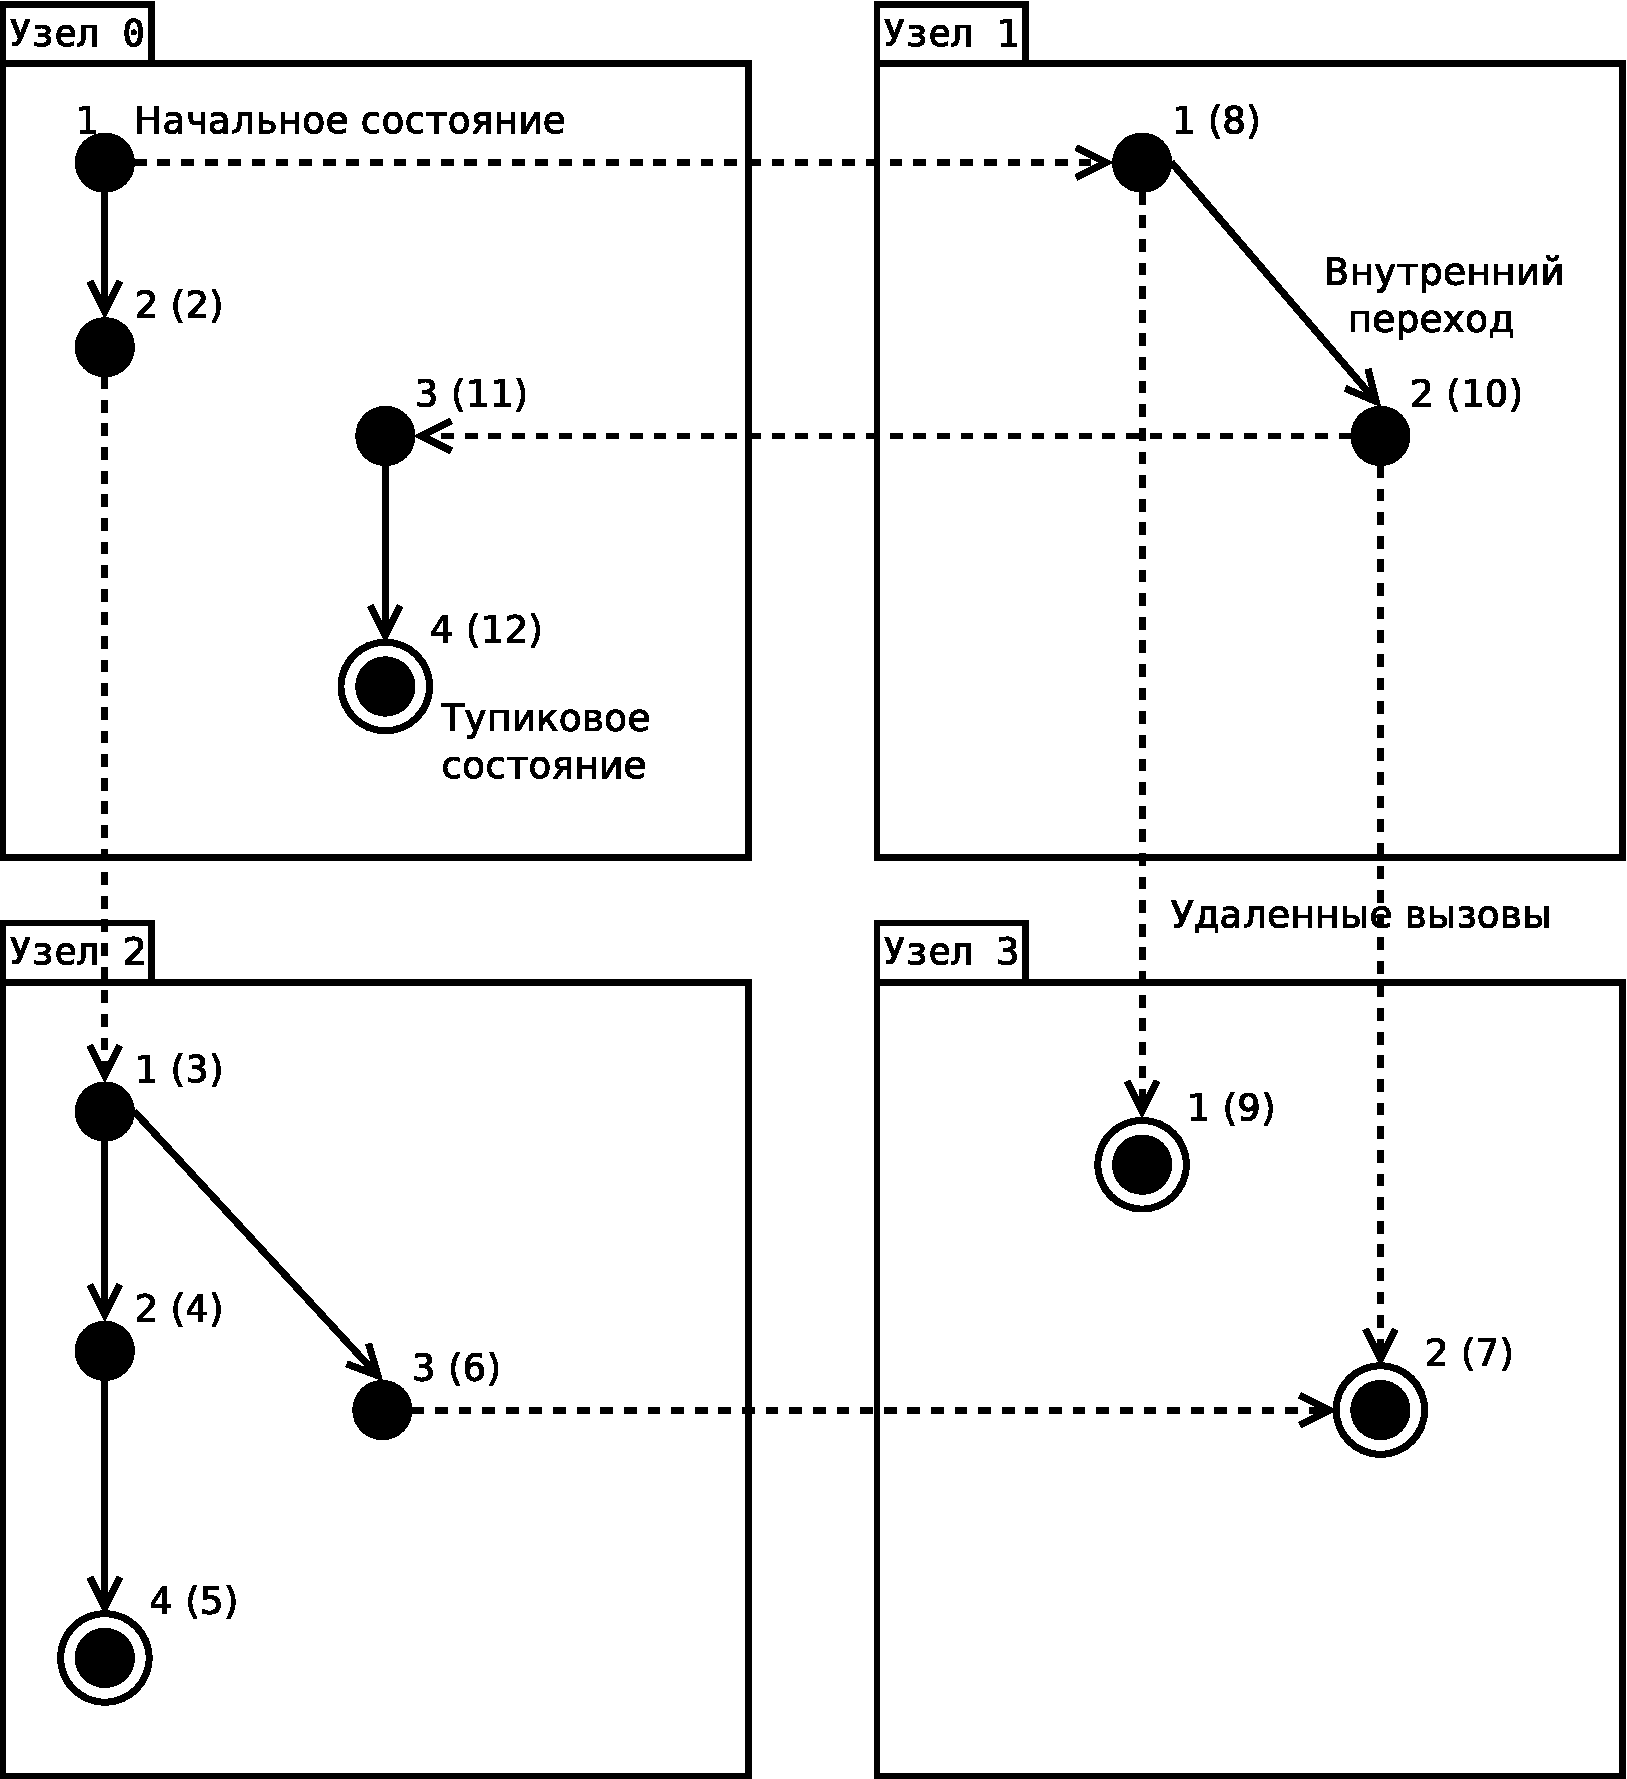
\includegraphics[width=0.6\textwidth]{../graphics/distr-generation}
  \caption{Пример работы распределенной генерации состояний}
  \label{fig:distr-generation}
\end{figure}

Одной из основных проблем распределенной генерации состояний является выбор функции распределения состояний между
узлами.

\section{Распределение состояний между узлами}
\label{sec:state-partition}

Функция распределения ставит в соответствие каждому состоянию индекс узла, отвечающего за хранение данного
состояний. Эта функция должна обладать следующими свойствами:

\begin{itemize}
\item она должна зависеть только от битового представления самого состояния, поскольку одно и то же состояние
  может генерироваться различными узлами в результате различных переходов;

\item она должна распределять состояния между узлами достаточно равномерно, в противном случае часть памяти у некоторых
  узлов будет простаивать;

\item она должна обладать свойством локальности относительно переходов между состояниями~--- по возможности новые
  состояния должны принадлежать тому же узлу, что и исходное.
\end{itemize}

Последнее условие имеет смысл лишь при втором подходе, <<распределенной генерации состояний>>, и позволяет уменьшить число
асинхронных удаленных вызовов между узлами.

Наиболее простым подходом является использование хэш-функции от битового представление состояния $s$ в качестве индекса
хранящего его узла. Это обеспечит первые два условия: если выбрана подходящая хэш-функция, распределение будет
достаточно равномерным. Однако, третье условие при этом не соблюдается, поскольку все новые состояния имеют равные шансы
принадлежать любому узлу независимо того, на каком узле они были сгенерированы.

Пусть число узлов~--- $N$, состояний~--- $S$, переходов между ними~--- $T$. В случае равномерного распределения
состояний между узлами вероятность того, что следующее состояние будет принадлежать текущему узлу, равняется
$1/N$. Следовательно, вероятность того, что потребуется удаленный вызов, равна $1 - 1/N$, а среднее число удаленных
вызовов в течение всей генерации составит
\begin{equation}
  \label{eq:rpc-partfull}
  Q = T (1 - \frac{1}{N}),
\end{equation}
что при больших значениях стремится к $T$.

Cтоль высокое число удаленных вызовов негативно отражаются на производительности, поэтому необходимо найти более удачную
функцию распределения состояний, которая бы удовлетворяла условию локальности. Одна из возможных идей предложена
в~\cite{LS99}: использовать хэш-код не от всего состояния $s$, а от некоторой его части $\tilde{s}$.

Битовое представление состояния в общем случае представляет собой набор значений переменных, описывающих состояние
отдельных компонент моделируемой системы и значения общих переменных, описывающих взаимодействие между ними.

Пусть $P$~--- число таких компонент (процессов в нотации Promela) в модели, $k$~--- среднее число компонент, состояние
которых меняется при переходе. Для языка Promela $1 \approx k < 2$ , поскольку взаимодействие между более чем двумя
процессами\footnote{Далее под словом <<процесс>> будет подразумеваться процесс в понимании Promela, т.е. компонент
  моделируемой системы.} нереализуемо, но для двух процессов есть возможность синхронной передачи сообщения, при которой
оба меняют свое состояние. Последняя возможность используется нечасто, поэтому для большинства моделей $k$ достаточно
близко к 1.

Таким образом, битовое представления состояния естественным образом разделяется на $(P+1)$ область, с учетом области
глобальных переменных. При этом $P$ из них меняются почти независимо друг от друга при условии $k \approx 1$, и в
качестве хэшируемого подсостояния $\tilde{s}$ можно выбрать первые (или произвольные) $\rho$ областей, хранящих
локальные состояния первых $\rho$ процессов.

Если предположить, что каждый процесс $p_i$ участвует примерно в равной доле переходов, то для произвольного наперед
заданного процесса вероятность участия в данном переходе составит $k/\rho$, а для $\rho$ процессов при $k \approx 1$
либо небольшом $\rho$~--- $\frac{k \rho}{P}$. При условии, что множество возможных локальных состояний процесса
отображается на множество узлов равномерным образом, вероятность удаленного вызова при изменении локального состояния
процесса (т.е. при его участии в переходе), по аналогии с предыдущими рассуждениями, составит $1 - 1/N$. Количество
удаленных вызовов во всей модели, таким образом, равняется
\begin{equation}
  \label{eq:rpc-partproc}
  Q_\rho = \frac{k \rho}{P} T (1 - \frac{1}{N})
\end{equation}
и с ростом $N$ стремится к $\frac{k \rho}{P} T$. При количестве процессов $P = 10$, $k = 1.1$ и $\rho = 2$, число
удаленных вызовов уменьшается примерно в 4 раза в сравнении с <<наивным>> подходом.

Выбор меньших значений $\rho$ приводит к меньшему числу удаленных вызовов, однако увеличивает неравномерность
распределения, поэтому его значение следует выбирать из баланса между требуемоей равномерностью распределения состояний
и выигрышем во времени за счет уменьшения числа вызовов.

Пусть $i$-ый процесс $p_i$ имеет $w_i$ возможных значений локального состояний, т.е. число допустимых комбинаций
значений его переменных составляет $w_i$. Объединение локальных состояний $\rho$ процессов тогда имеет не более $W_\rho
= \prod_{i=1}^{\rho}{w_i}$ возможных значений. Число значений может быть меньше $W_\rho$, поскольку в общем случае не
все комбинации являются допустимыми. Значение $\rho$ должно обеспечивать условие $W_\rho \gg N$, иначе, особенно при
$W_\rho \approx N$, распределение будет неравномерным даже при удачном выборе хэш-функции, а при $W_\rho < N$ память
некоторых узлов не будет использоваться вообще, так как число возможных значений хэш-функции будем меньше числа узлов.

\section{Результаты}
\label{sec:experim}

Создано программное средство для параллельной проверки состояний с распределенной генерацией, поддерживающий
подмножество языка Promela для описания модели. Для задания проверямых утверждений поддерживается подмножество LTL,
допускающее формулы $\mathbf{AG}~x$ и $\mathbf{AF}~x$, где $x$ может содержать локальные переменные процессов (включая
счетчик команд) и глобальные переменные. На практике данное подмножество LTL реализовано при помощи встроенной в Promela
функции \texttt{assert} и поиска тупиковых состояний.

В разработанном средстве поддерживаются основные возможности языка Promela, такие как асинхронные каналы,
пользовательские типа данных, \texttt{atomic} и \texttt{d\_step}~\cite{SpinRoot}.

Исходная модель на Promela считывается и транслируется во внутренний граф команд для каждого процесса, который затем
минимизируется. С целью достижения скорости генерации состояний, сравнимой со скоростью SPIN, по полученным графам
команд генерируется код на языке~C, выполняющий вычисление функции переходов модели $Next(s) = \{s': R(s, s')\}$ и
функции проверки состояний $Assert(s): S \rightarrow \{0, 1\}$. Функциональная схема данного процесса приведена на
рис.~\ref{fig:stategen-idef0-b0}.

\begin{figure}[ht]
  \centering
  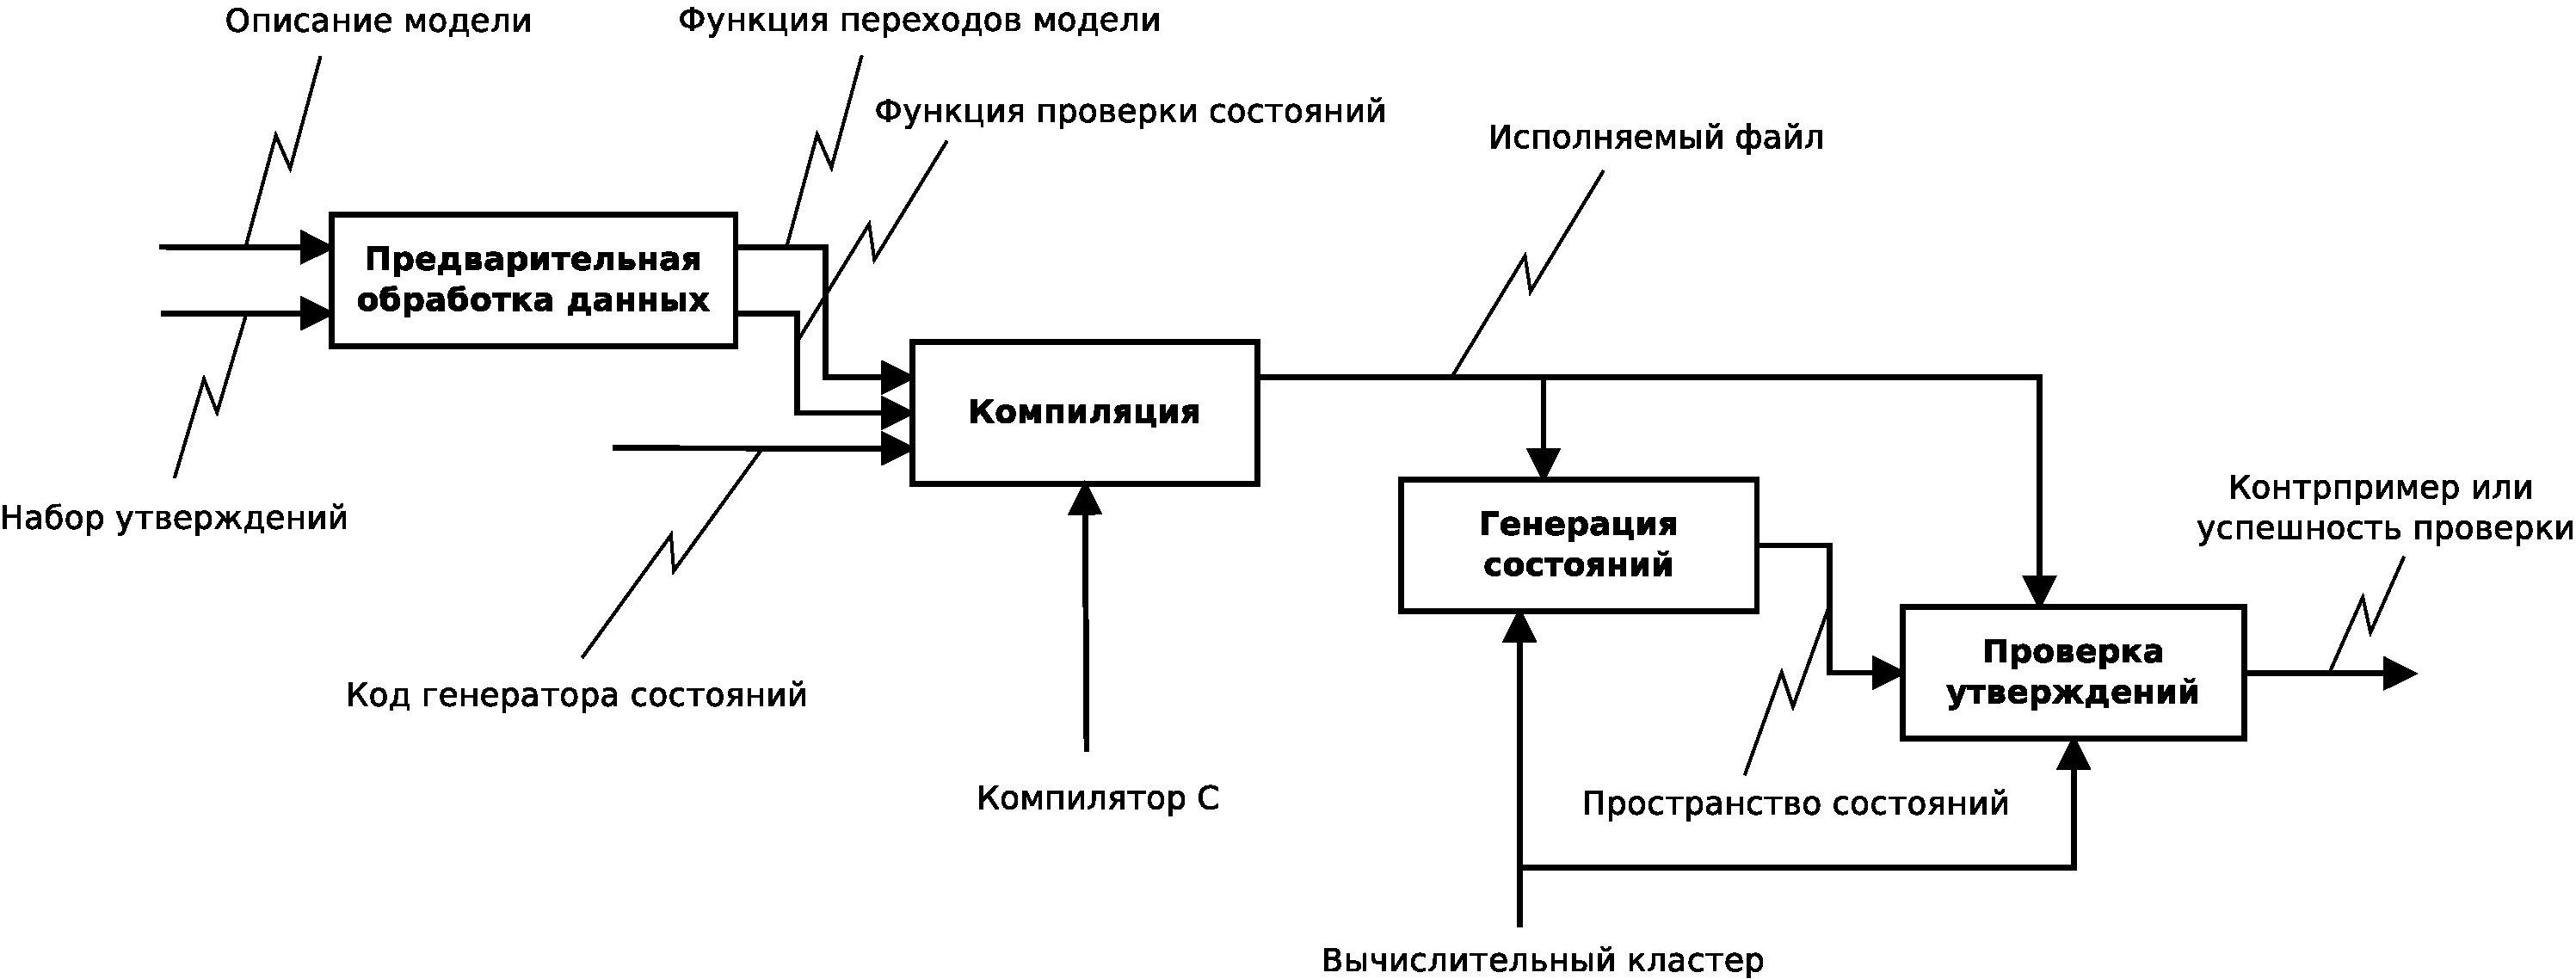
\includegraphics[width=\textwidth]{../graphics/stategen-idef0-b0}
  \caption{Функциональная схема процесса генерации кода по описанию модели}
  \label{fig:stategen-idef0-b0}
\end{figure}

В качестве платформы для параллельных вычислений использовался стандарт MPI, выбранный в силу его распространенности
среди кластерного ПО и поддержки широкого набора языков.

Исходными данными служат две модели: алгоритм выбора лидера и <<обедающие философы>> с числом компонент $P = 6$. Для
проведения экспериментов использовался кластер из 20 узлов, имеющих 4 Гб ОЗУ и 4 ЦПУ Intel\,Xeon\,5120~1.86 ГГц каждый.

Результаты экспериментов по сравнению предлагаемого распределения с $\rho = 1$ и $\rho = 2$ с наивным представлены на
табл.~\ref{tab:election-results} и~\ref{tab:philo-results}. Приведены следующие величины:

\begin{itemize}
\item доля вызовов среди переходов~--- отношение числа удаленных вызовов (суммарно на всех узлах) к числу переходов $T$;

\item неравномерность распределения~--- отношение среднеквадратичного отклонения к среднему для последовательности $m_1
  m_2 \ldots m_N$, где $m_i$~--- число состояний, хранимых узлом $i$;

\item время простоя при ожидании сообщений от других узлов (сетевые задержки);

\item общее время работы.
\end{itemize}

\begin{table}[htb]
  \centering
  \begin{tabular}{|c|c|c|c|c|}
    \hline
    $\rho$ & Доля вызовов        & Неравномерность   & Время простоя, & Общее время работы, \\ \hline
           & среди переходов, \% & распределения, \% & сек            & сек                 \\ \hline
    1      & 16                  & \textbf{66.3}     & 29             & 43                  \\ \hline
    2      & 36                  & 12.8              & 65             & 84                  \\ \hline
    ---    & \textbf{87}         & 0.1               & \textbf{127}   & \textbf{164}        \\ \hline
  \end{tabular}
  \caption{Сравнение распределений (алгоритм выбора лидера)}
  \label{tab:election-results}
\end{table}

\begin{table}[htb]
  \centering
  \begin{tabular}{|c|c|c|c|c|}
    \hline
    $\rho$ & Доля вызовов        & Неравномерность   & Время простоя, & Общее время работы, \\ \hline
           & среди переходов, \% & распределения, \% & сек            & сек                 \\ \hline
    1      & 17                  & \textbf{89.4}     & 3              & 14                  \\ \hline
    2      & 35                  & 29.6              & 7              & 21                  \\ \hline
    ---    & \textbf{88}         & 0.1               & \textbf{50}    & \textbf{75}         \\ \hline
  \end{tabular}
  \caption{Сравнение распределений (<<обедающие философы>>)}
  \label{tab:philo-results}
\end{table}

Проблемные значения выделены жирным начертанием.

Из результатов можно сделать следующие выводы:

\begin{enumerate}
\item выбор распределения между узлами важен, поскольку время простоя за счет удаленных вызовов составляет существенного
  часть от времени выполнения;

\item при <<наивном>> подходе к распределению состояний число удаленных вызовов близко к числу всех переходов, как и следует
  из~\eqref{eq:rpc-partfull};

\item предлагаемый способ распределения состояний по первым $\rho$ процессам позволяет уменьшить число удаленных вызовов
  и время выполнения в сравнении с <<наивным>> подходом в соответствии с~\eqref{eq:rpc-partproc};

\item необходим подбор параметра $\rho$ в соответствии со свойствами проверямой модели ($P, w_i$) для обеспечения
  требуемого уровня равномерности распределения состояний; в частности, значения $\rho = 1$ в приведенных экспериментах
  оказалось недостаточно, поскольку неравномерность до 90\% означает, что большая часть памяти некоторых узлов не
  используется вообще.
\end{enumerate}

\section{Заключение}
\label{sec:conclusion}

Использование параллельной генерации состояний дискретных детерминированных моделей при проверке их соответствия
спецификациям позволяет выполнять верификацию моделей на несколько порядков большего размера, чем позволяют аналогичные
подходы с последовательной генерацией. Одним из наиболее важных факторов является функция распределения хранимых
состояний между узлам, правильный выбор которой, как подтверждают эксперименты, позволяет в несколько раз ускорить
верификацию.

\bibliographystyle{../thesis/gost780u}
\bibliography{../thesis/thesis}

\end{document}

%%% Local Variables:
%%% mode: latex
%%% TeX-master: t
%%% fill-column: 120
%%% End:
